\bigskip
\begin{center}
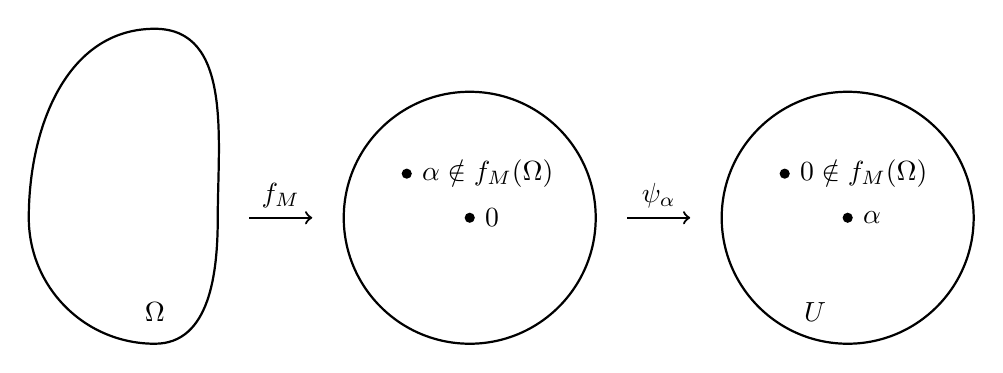
\begin{tikzpicture}[scale=.8]
    %Omega
    \draw[thick] (-1,0) to[out=90,in=180] (1,3) to[out=0,in=90] (2,0) 
    to[out=-90,in=0] (1,-2) to[out=180,in=-90] cycle;
    \node at (1,-1.5) {$\Omega$};

    % f_M
    \draw[->,thick] (2.5,0) -- (3.5,0) node[midway,above] {$f_M$};

    % middle disk
    \begin{scope}[shift={(6,0)}]
        \draw[thick] (0,0) circle (2);
        \node[fill,circle,inner sep=1.3pt,label=right:$\alpha \notin f_M(\Omega)$] (a1) at (-1,0.7) {};
        \node[fill,circle,inner sep=1.3pt,label=right:$0$] (o1) at (0,0) {};
        \node[label=right:$\disk$] at (-1,-1.5) {};
%\draw[<->] (a1) to[out=-100,in=170] node[below=4pt,pos=0.5] {$\psi_{\alpha}$} (o1);
    \end{scope}

    % Arrow to second disk
    \draw[->,thick] (8.5,0) -- (9.5,0) node[midway,above] {$\psi_{\alpha}$};

    % right disk
    \begin{scope}[shift={(12,0)}]
        \draw[thick] (0,0) circle (2);
        \node[fill,circle,inner sep=1.3pt,label= right:$0 \notin f_M(\Omega)$] at (-1,0.7) {};
        \node[fill,circle,inner sep=1.3pt,label=right:$\alpha$] at (0,0) {};
        \node[label=right:$U$] at (-1,-1.5) {};
    \end{scope}

\end{tikzpicture}
\end{center}
\bigskip